%!TEX root = ../thesis.tex
% ******************************* Thesis Appendix D ********************************

\chapter{dL/dx vs. dE/dx plots} \label{appendixD:dldxVsDedxPlots}

\begin{figure}[htbp]
 \centering
 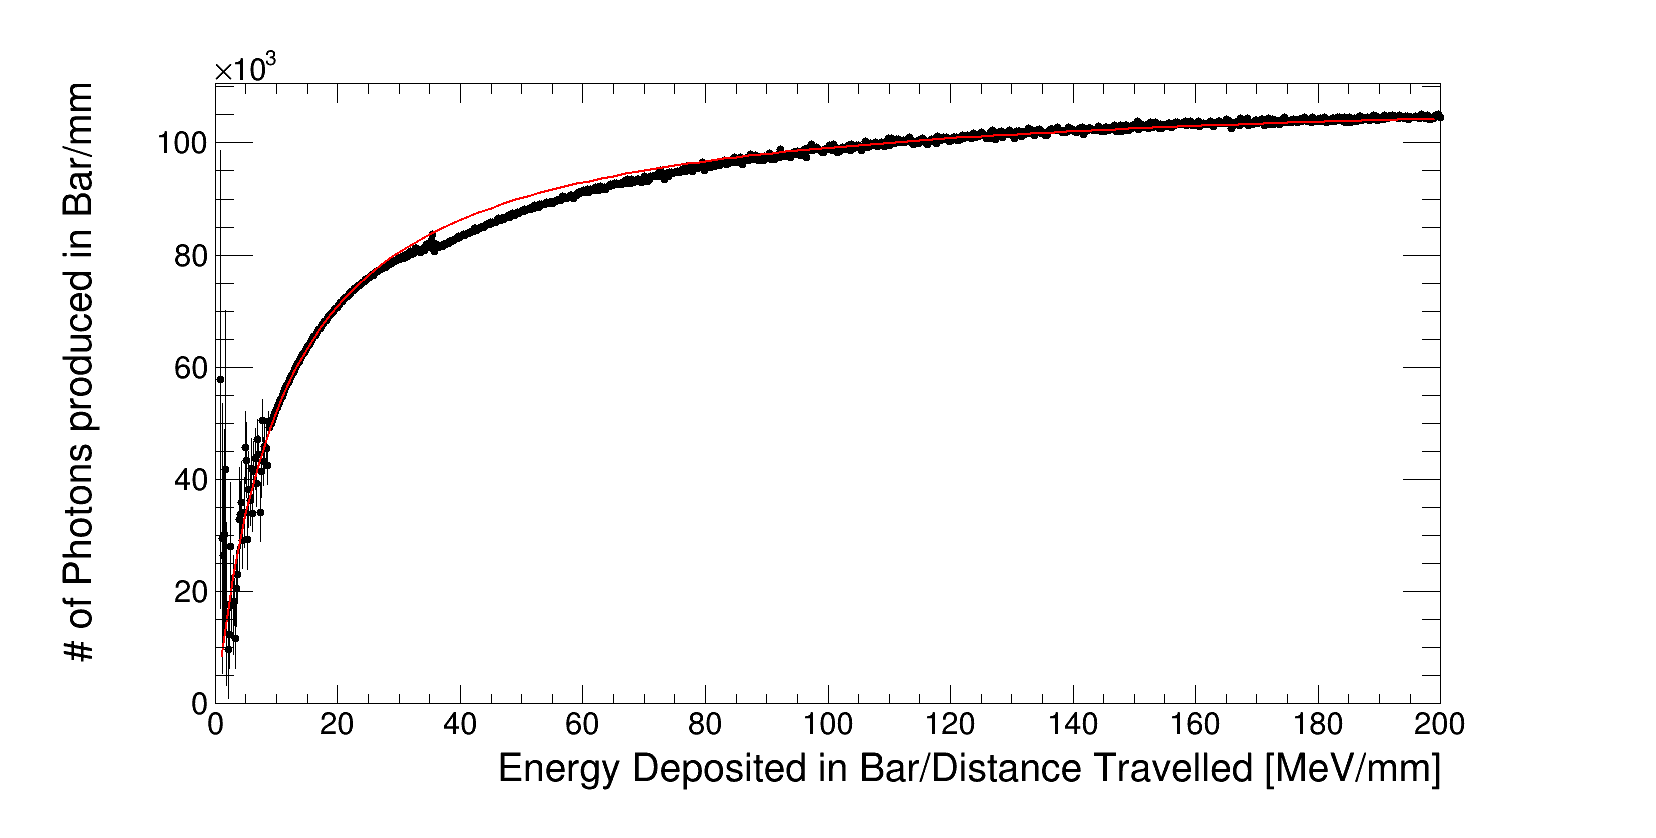
\includegraphics[width=\linewidth]{Appendix4/Figs/newNewDldxVsDeDx/alphaDeDxDlDx.png}
 \captionof{figure}[dL/dx vs dE/dx ``slice'' Birks' model approximation for alpha particles.]{dL/dx vs dE/dx fit using the approximation $\Delta L$/$\Delta x$ vs $\Delta E$/$\Delta x$ from the ``slice model'' simulation of scintillator for 2E6 simulated alpha particles, $\chi^2$/NDF = 98.3163.} 
 \label{fig:slice_Alpha_dl_dx} 
\end{figure}

\begin{figure}[htbp]
 \centering
 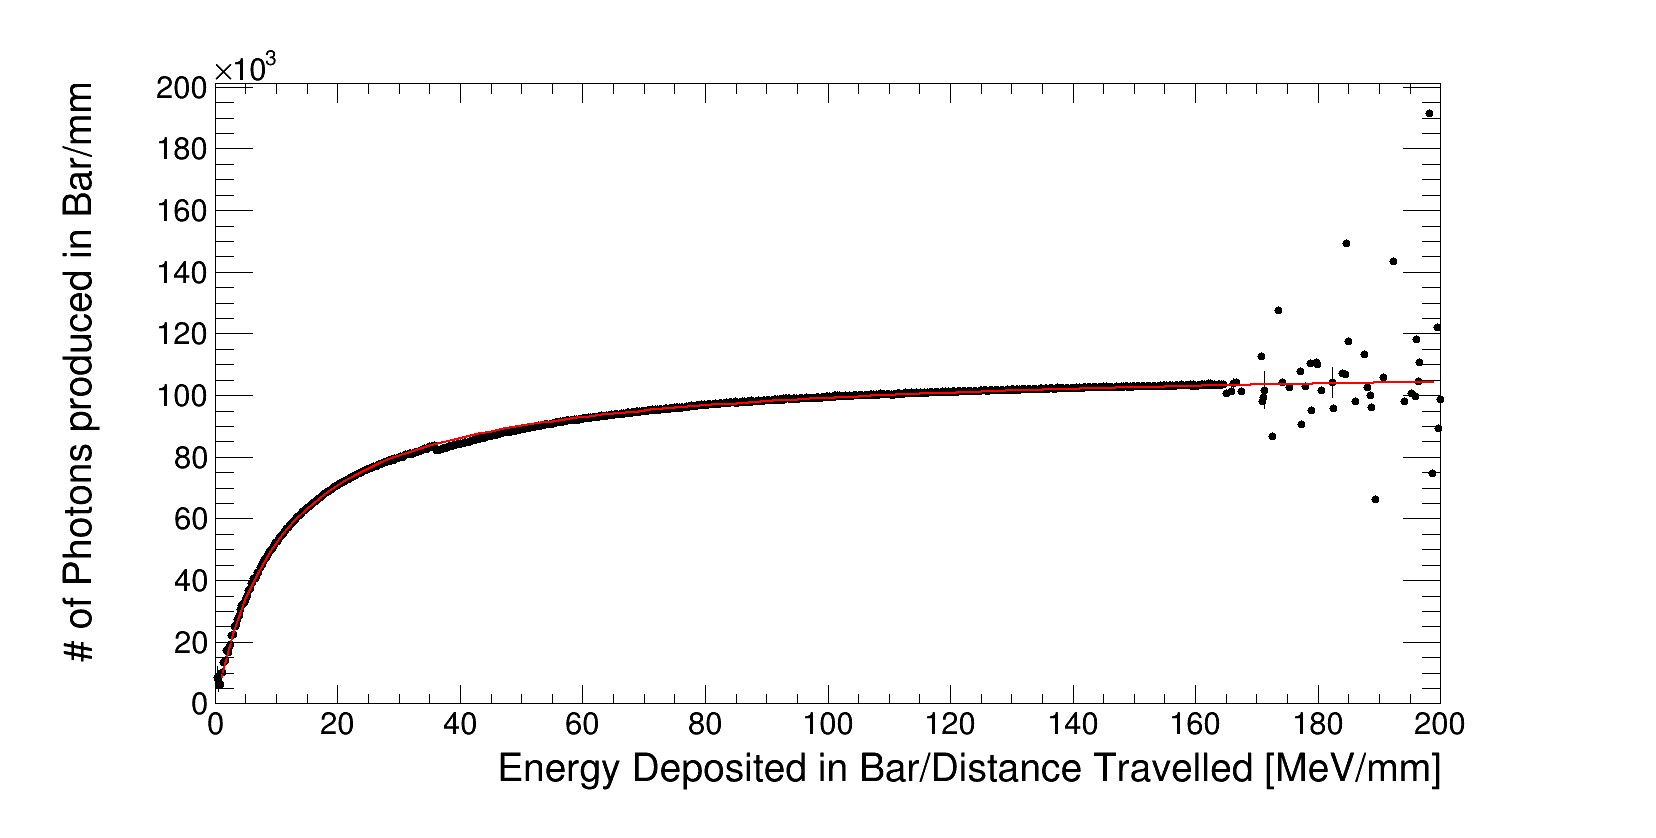
\includegraphics[width=\linewidth]{Appendix4/Figs/newNewDldxVsDeDx/antiAlphaDeDxDlDx.png}
 \captionof{figure}[dL/dx vs dE/dx ``slice'' Birks' model approximation for anti-alpha particles.]{dL/dx vs dE/dx fit using the approximation $\Delta L$/$\Delta x$ vs $\Delta E$/$\Delta x$ from the ``slice model'' simulation of scintillator for 2E6 simulated $\Bar{\alpha}$ particles, $\chi^2$/NDF = 85.7297.} 
 \label{fig:slice_AAlpha_dl_dx}
\end{figure}

\begin{figure}[htbp]
 \centering
 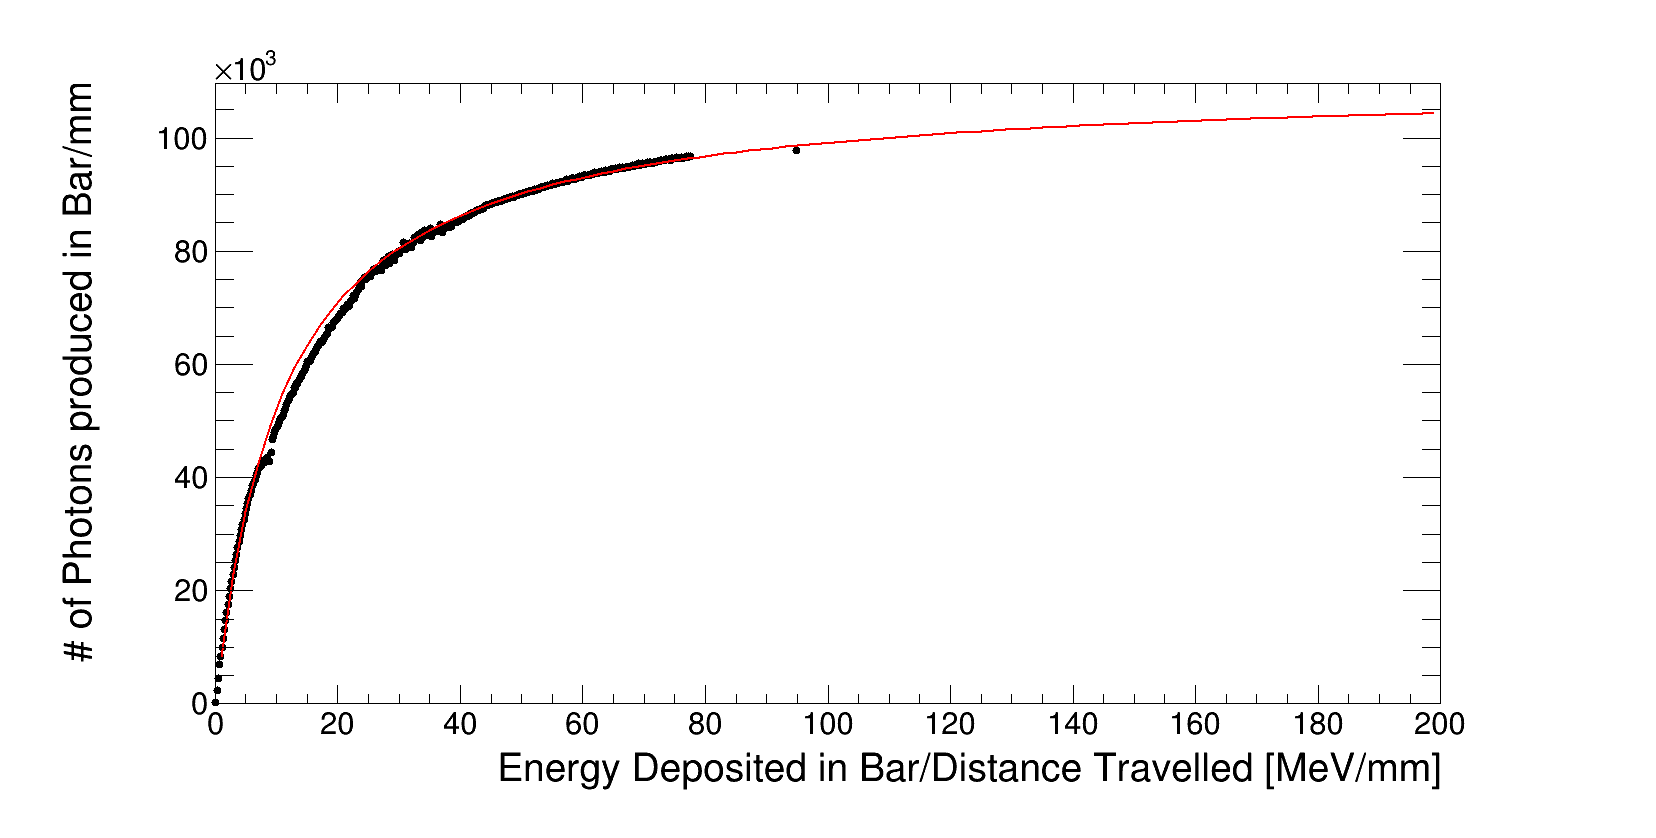
\includegraphics[width=\linewidth]{Appendix4/Figs/newNewDldxVsDeDx/protonDeDxDlDx.png}
 \captionof{figure}[dL/dx vs dE/dx ``slice'' Birks' model approximation for protons.]{dL/dx vs dE/dx fit using the approximation $\Delta L$/$\Delta x$ vs $\Delta E$/$\Delta x$ from the ``slice model'' simulation of scintillator for 2E6 simulated proton particles, $\chi^2$/NDF = 297.246.} 
 \label{fig:slice_Proton_dl_dx}
\end{figure}

\begin{figure}[htbp]
 \centering
 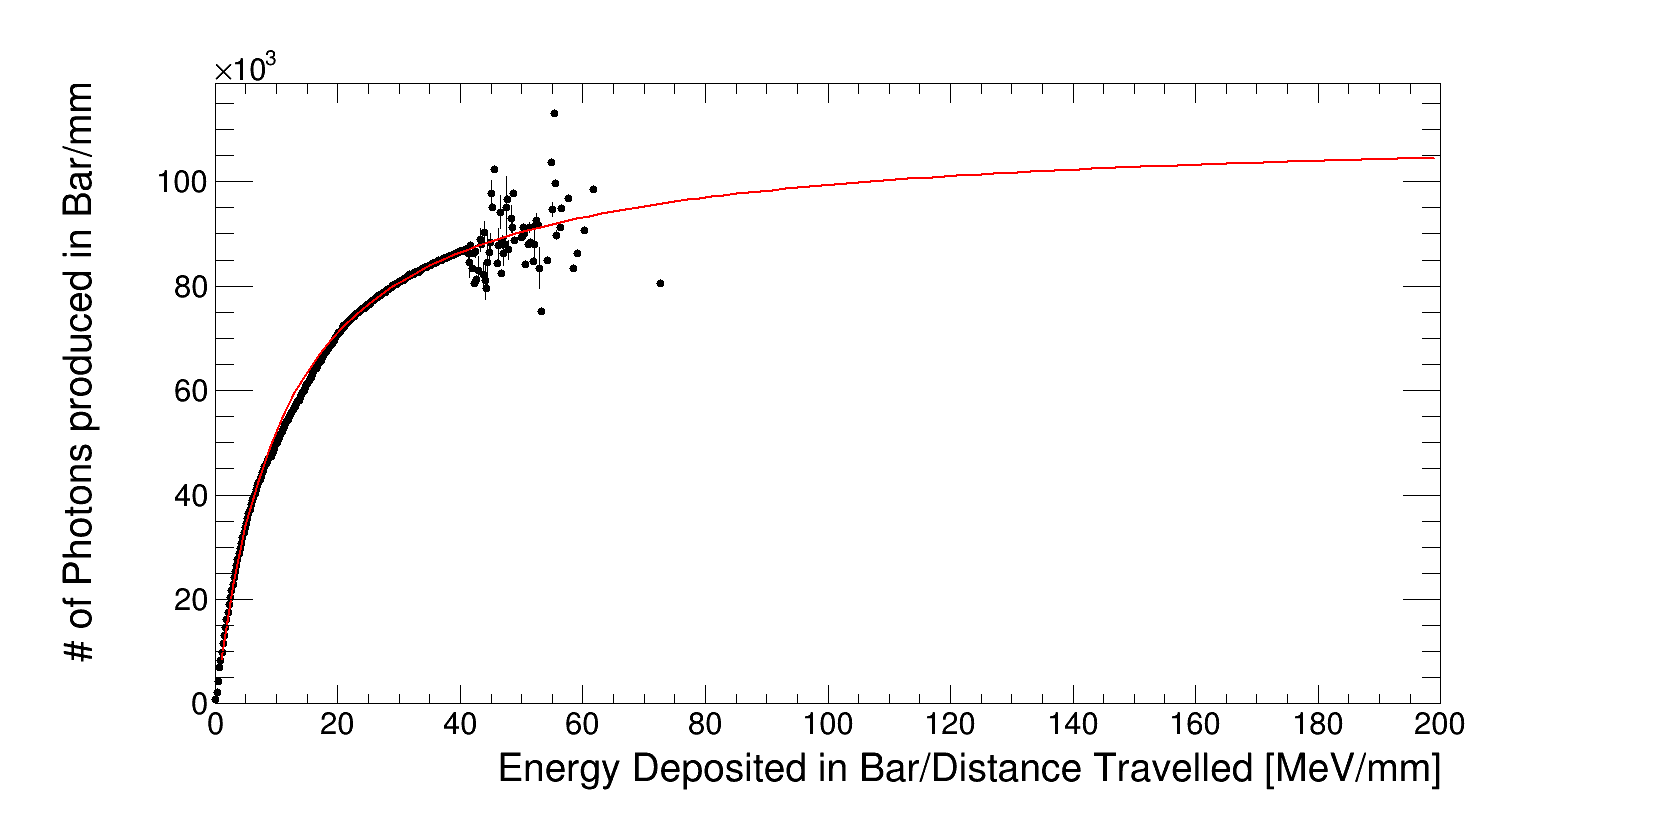
\includegraphics[width=\linewidth]{Appendix4/Figs/newNewDldxVsDeDx/antiProtonDeDxDlDx.png}
 \captionof{figure}[dL/dx vs dE/dx ``slice'' Birks' model approximation for anti-protons.]{dL/dx vs dE/dx fit using the approximation $\Delta L$/$\Delta x$ vs $\Delta E$/$\Delta x$ from the ``slice model'' simulation of scintillator for 2E6 simulated anti-proton particles, $\chi^2$/NDF = 607.475.} 
 \label{fig:slice_AProton_dl_dx}
\end{figure}

\begin{figure}[htbp]
 \centering
 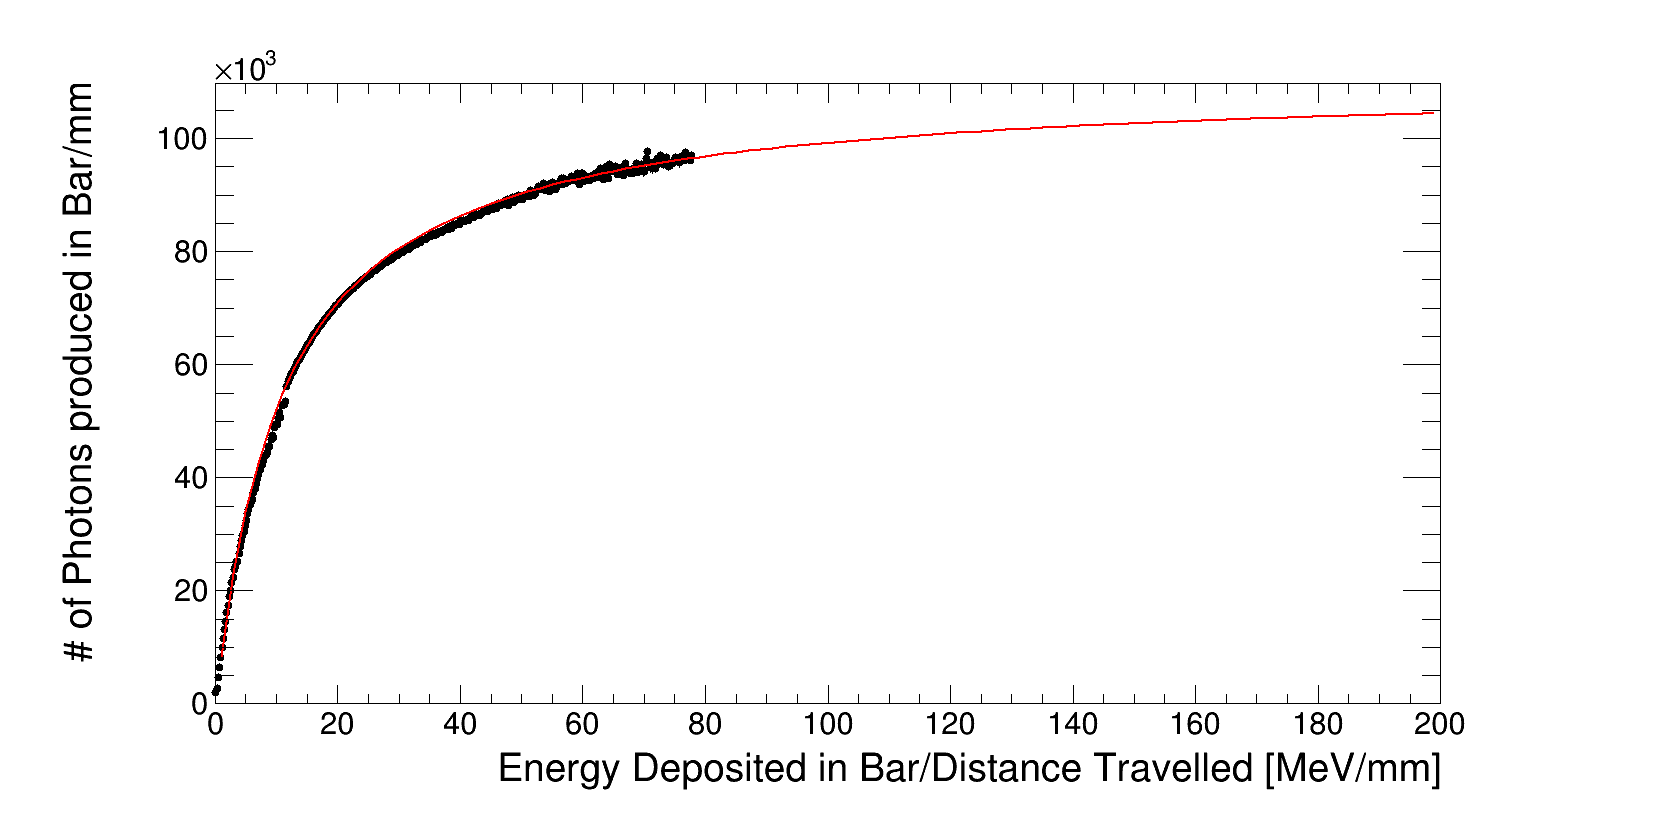
\includegraphics[width=\linewidth]{Appendix4/Figs/newNewDldxVsDeDx/pi+DeDxDlDx.png}
 \captionof{figure}[dL/dx vs dE/dx ``slice'' Birks' model approximation for positive pion particles.]{dL/dx vs dE/dx fit using the approximation $\Delta L$/$\Delta x$ vs $\Delta E$/$\Delta x$ from the ``slice model'' simulation of scintillator for 2E6 simulated $\pi^+$ particles, $\chi^2$/NDF = 9762.33.} 
 \label{fig:slice_APiPlus_dl_dx}
\end{figure}

\begin{figure}[htbp]
 \centering
 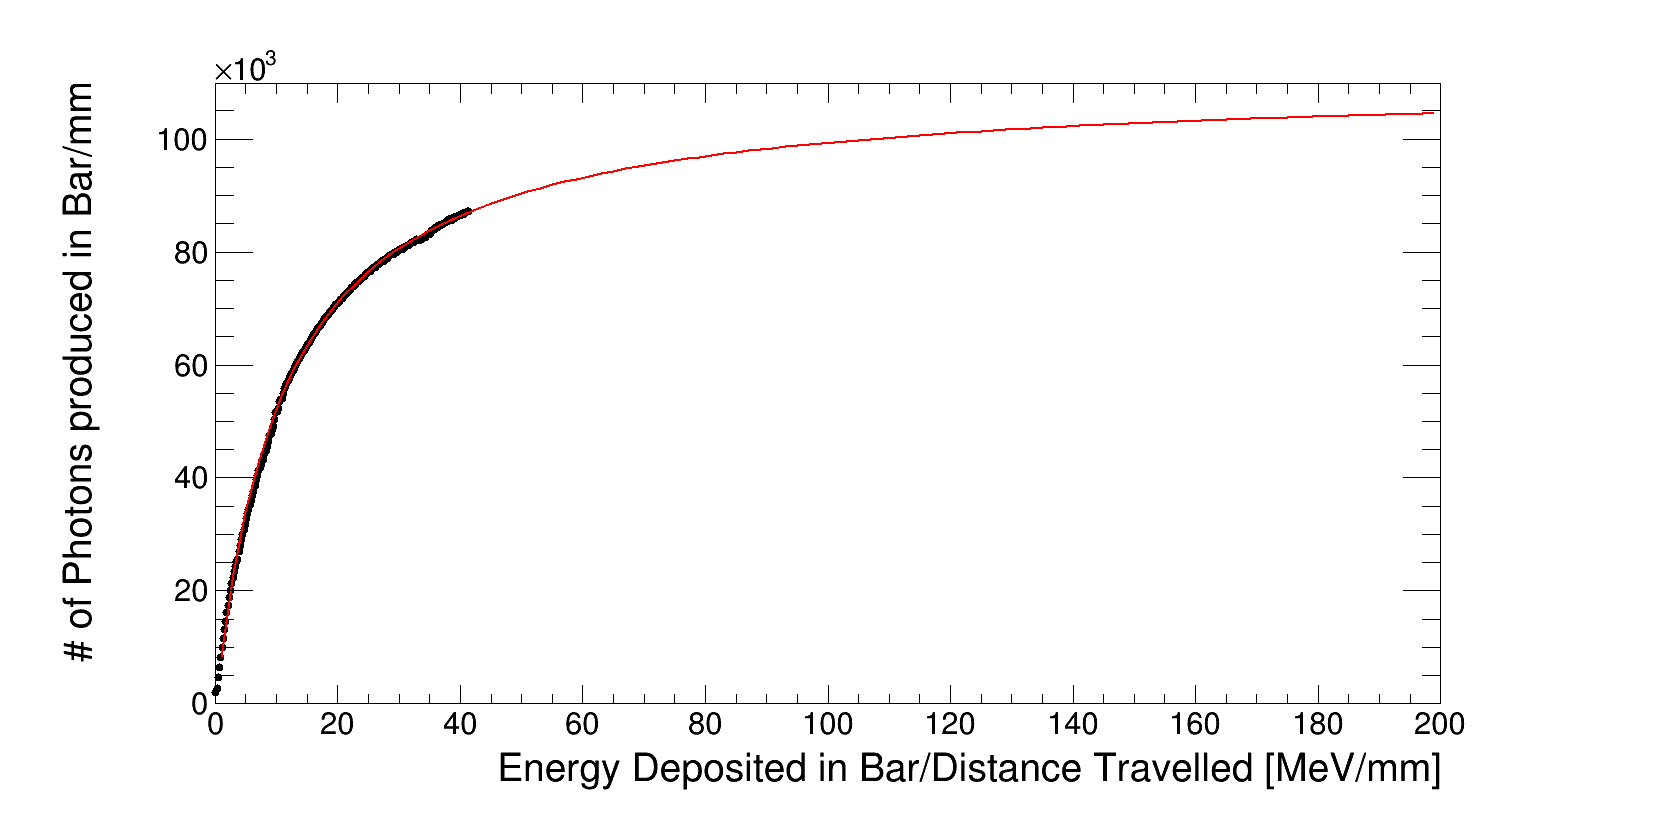
\includegraphics[width=\linewidth]{Appendix4/Figs/newNewDldxVsDeDx/pi-DeDxDlDx.png}
 \captionof{figure}[dL/dx vs dE/dx ``slice'' Birks' model approximation for negative pion particles.]{dL/dx vs dE/dx fit using the approximation $\Delta L$/$\Delta x$ vs $\Delta E$/$\Delta x$ from the ``slice model'' simulation of scintillator for 2E6 simulated $\pi^-$ particles, $\chi^2$/NDF = 13193.4.} 
 \label{fig:slice_APiMinus_dl_dx}
\end{figure}

\begin{figure}[htbp]
 \centering
 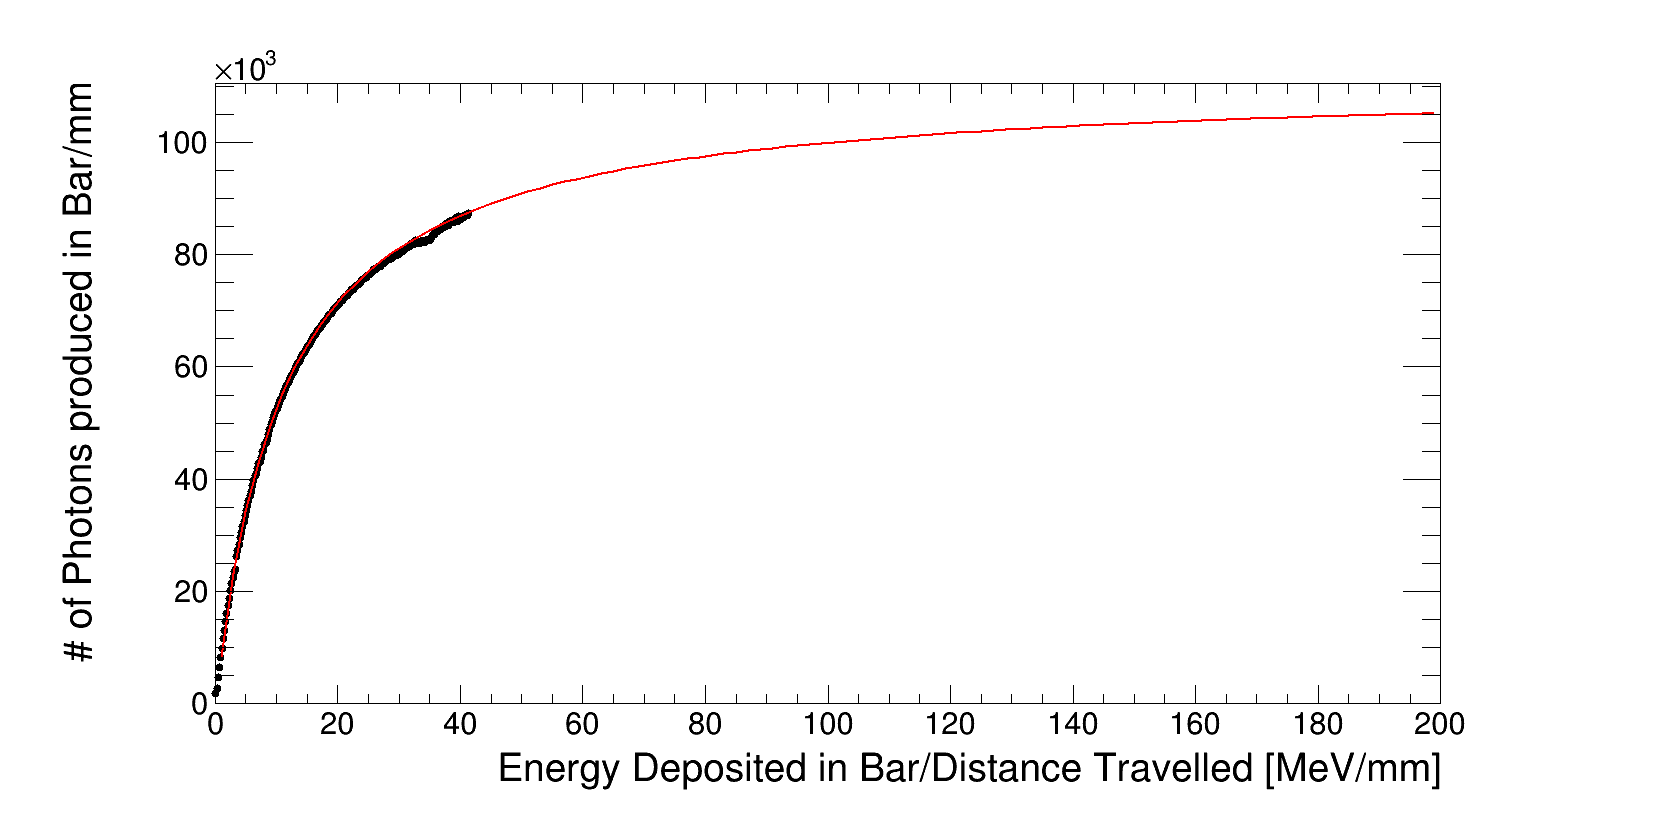
\includegraphics[width=\linewidth]{Appendix4/Figs/newNewDldxVsDeDx/muonDeDxDlDx.png}
 \captionof{figure}[dL/dx vs dE/dx ``slice'' Birks' model approximation for muons.]{dL/dx vs dE/dx fit using the approximation $\Delta L$/$\Delta x$ vs $\Delta E$/$\Delta x$ from the ``slice model'' simulation of scintillator for 2E6 simulated $\mu^-$ particles, $\chi^2$/NDF = 42026.8.} 
 \label{fig:slice_Muon_dl_dx}
\end{figure}

\begin{figure}[htbp]
 \centering
 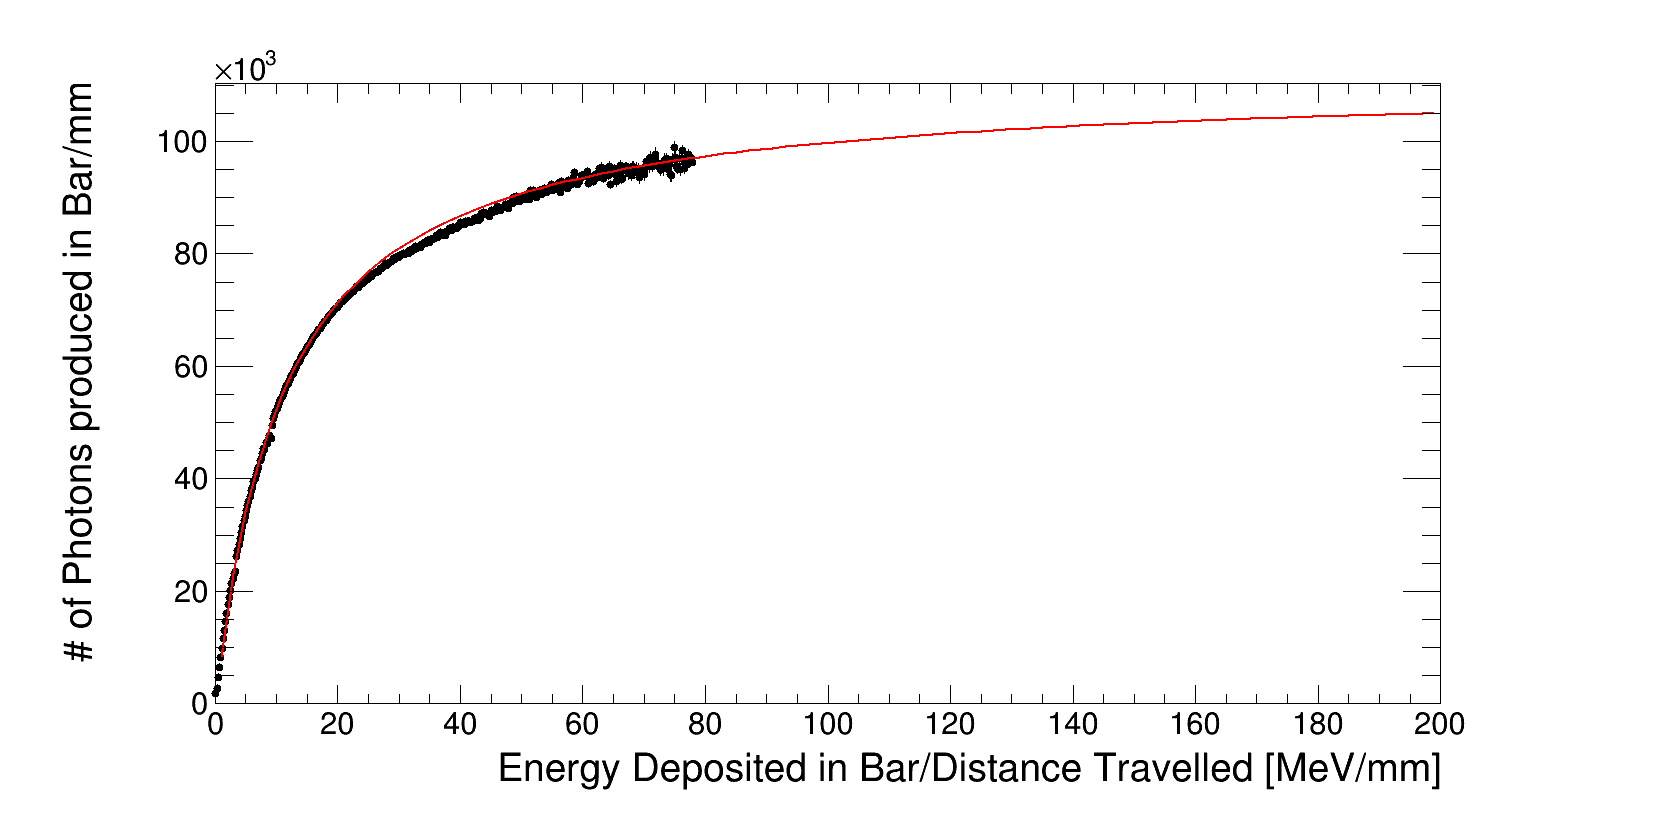
\includegraphics[width=\linewidth]{Appendix4/Figs/newNewDldxVsDeDx/antiMuonDeDxDlDx.png}
 \captionof{figure}[dL/dx vs dE/dx ``slice'' Birks' model approximation for anti-muons.]{dL/dx vs dE/dx fit using the approximation $\Delta L$/$\Delta x$ vs $\Delta E$/$\Delta x$ from the ``slice model'' simulation of scintillator for 2E6 simulated $\mu^+$ particles, $\chi^2$/NDF = 23874.9.} 
 \label{fig:slice_AMuon_dl_dx}
\end{figure}

\begin{figure}[htbp]
 \centering
 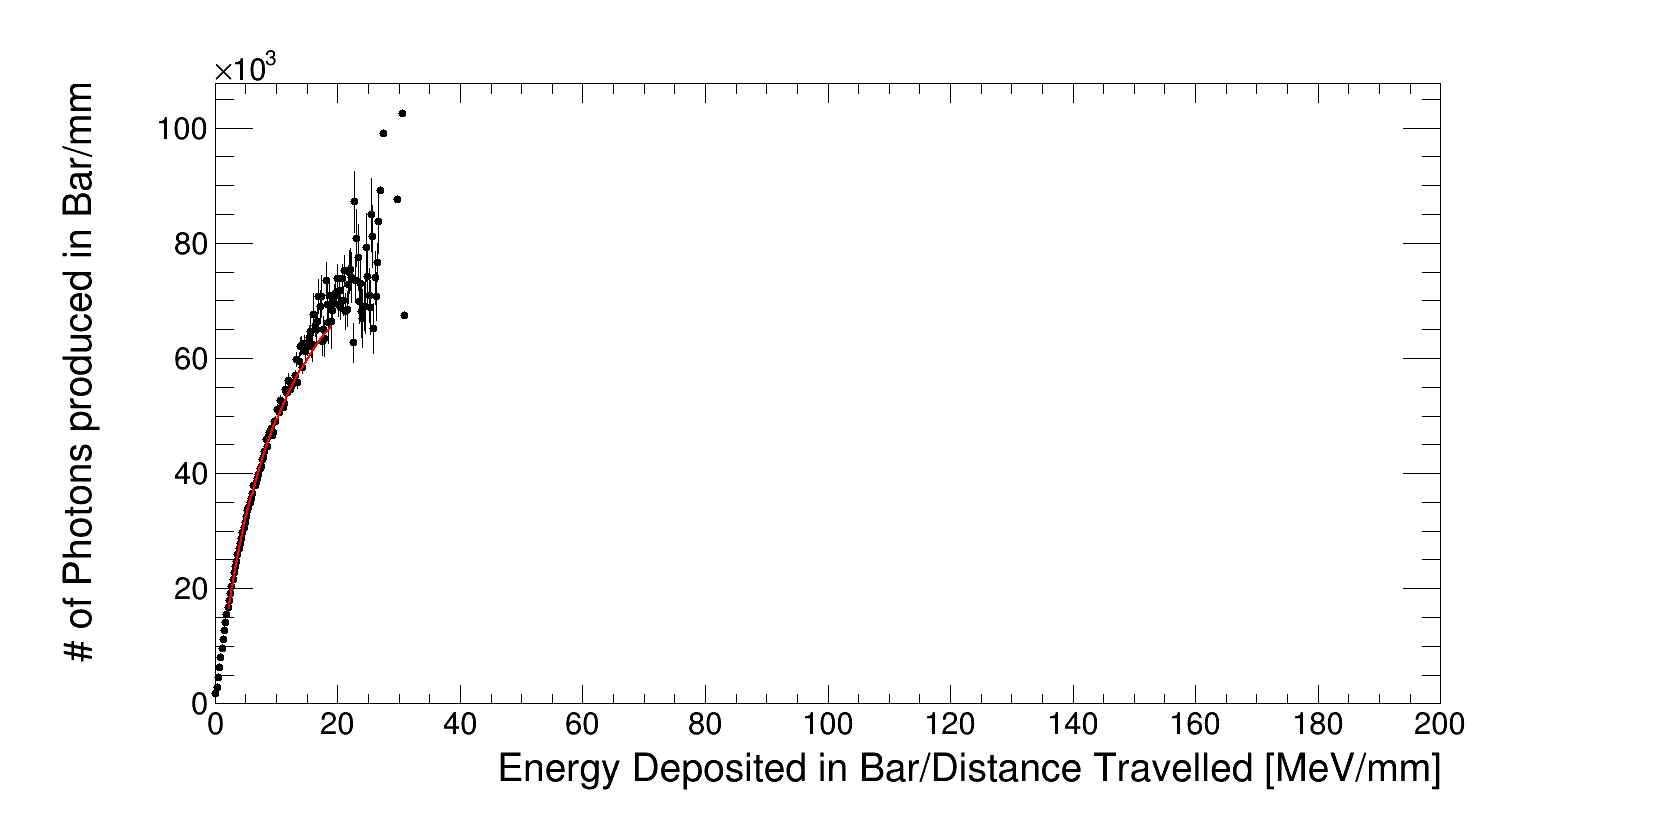
\includegraphics[width=\linewidth]{Appendix4/Figs/newNewDldxVsDeDx/electronDeDxDlDx.png}
 \captionof{figure}[dL/dx vs dE/dx ``slice'' Birks' model approximation for electrons.]{dL/dx vs dE/dx fit using the approximation $\Delta L$/$\Delta x$ vs $\Delta E$/$\Delta x$ from the ``slice model'' simulation of scintillator for 2E7 simulated $e^-$ particles, $\chi^2$/NDF = 13.4511. The Birks fit is used for 2\,MeV -- 19\,MeV. } 
 \label{fig:slice_Electron_dl_dx}
\end{figure}

\begin{figure}[htbp]
 \centering
 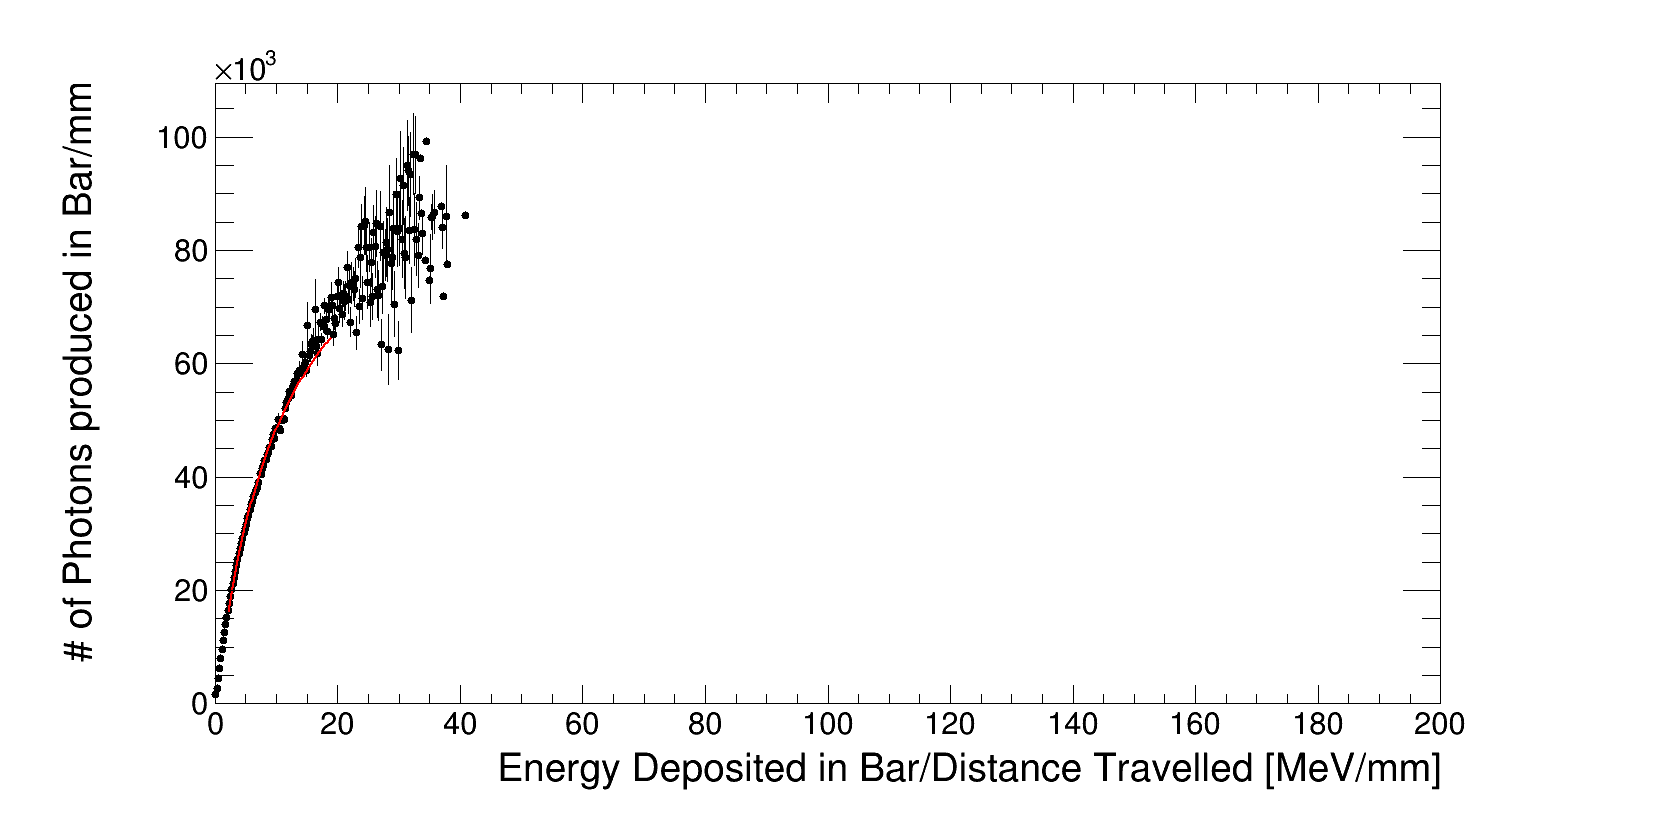
\includegraphics[width=\linewidth]{Appendix4/Figs/newNewDldxVsDeDx/positronDeDxDlDx.png}
 \captionof{figure}[dL/dx vs dE/dx ``slice'' Birks' model approximation for positrons.]{dL/dx vs dE/dx fit using the approximation $\Delta L$/$\Delta x$ vs $\Delta E$/$\Delta x$ from the ``slice model'' simulation of scintillator for 2E7 simulated $e^+$ particles, $\chi^2$/NDF = 26.33.55. The Birks fit is used for 2\,MeV -- 19\,MeV. } 
 \label{fig:slice_Positron_dl_dx}
\end{figure}

\begin{figure}[htbp]
 \centering
 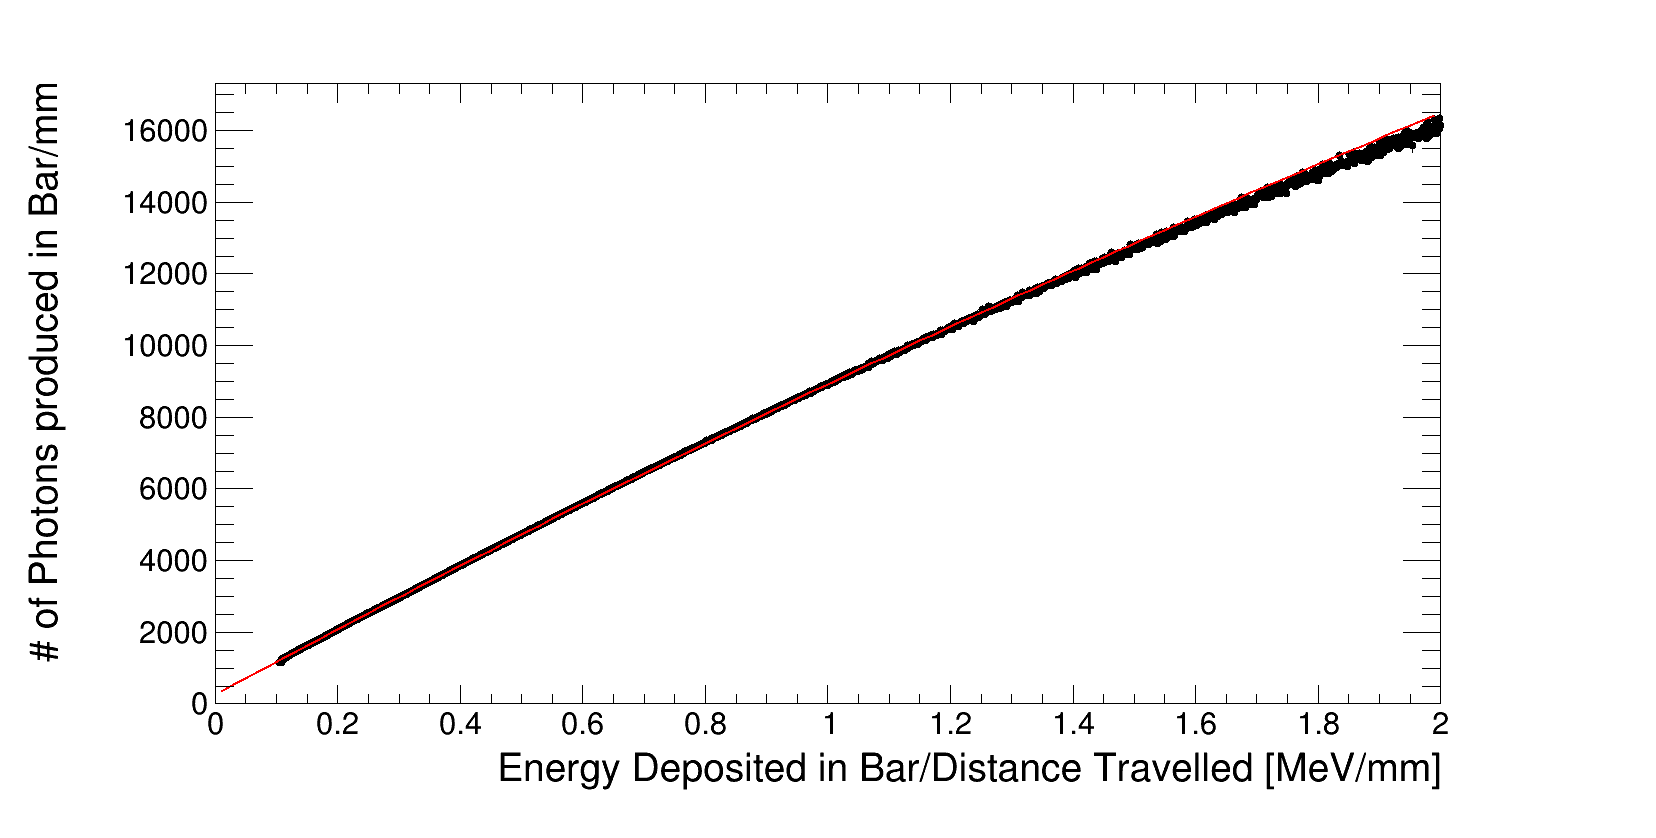
\includegraphics[width=\linewidth]{Appendix4/Figs/newNewDldxVsDeDx/e-_dedxVsdldxFitFine.png}
 \captionof{figure}[dL/dx vs dE/dx 2$^\textrm{nd}$ order polynomial ``slice'' model approximation for electrons.]{dL/dx vs dE/dx fit using the approximation $\Delta L$/$\Delta x$ vs $\Delta E$/$\Delta x$ from the ``slice model'' simulation of scintillator for 2E7 simulated $e^-$ particles, $\chi^2$/NDF = 39.9469. A 2 $^\textrm{nd}$ order polynomial fit is used between 0\,MeV -- 2\,MeV to accurately quantify the effect at low values of dE/dx. } 
 \label{fig:slice_Electron_fine_dl_dx}
\end{figure}

\begin{figure}[htbp]
 \centering
 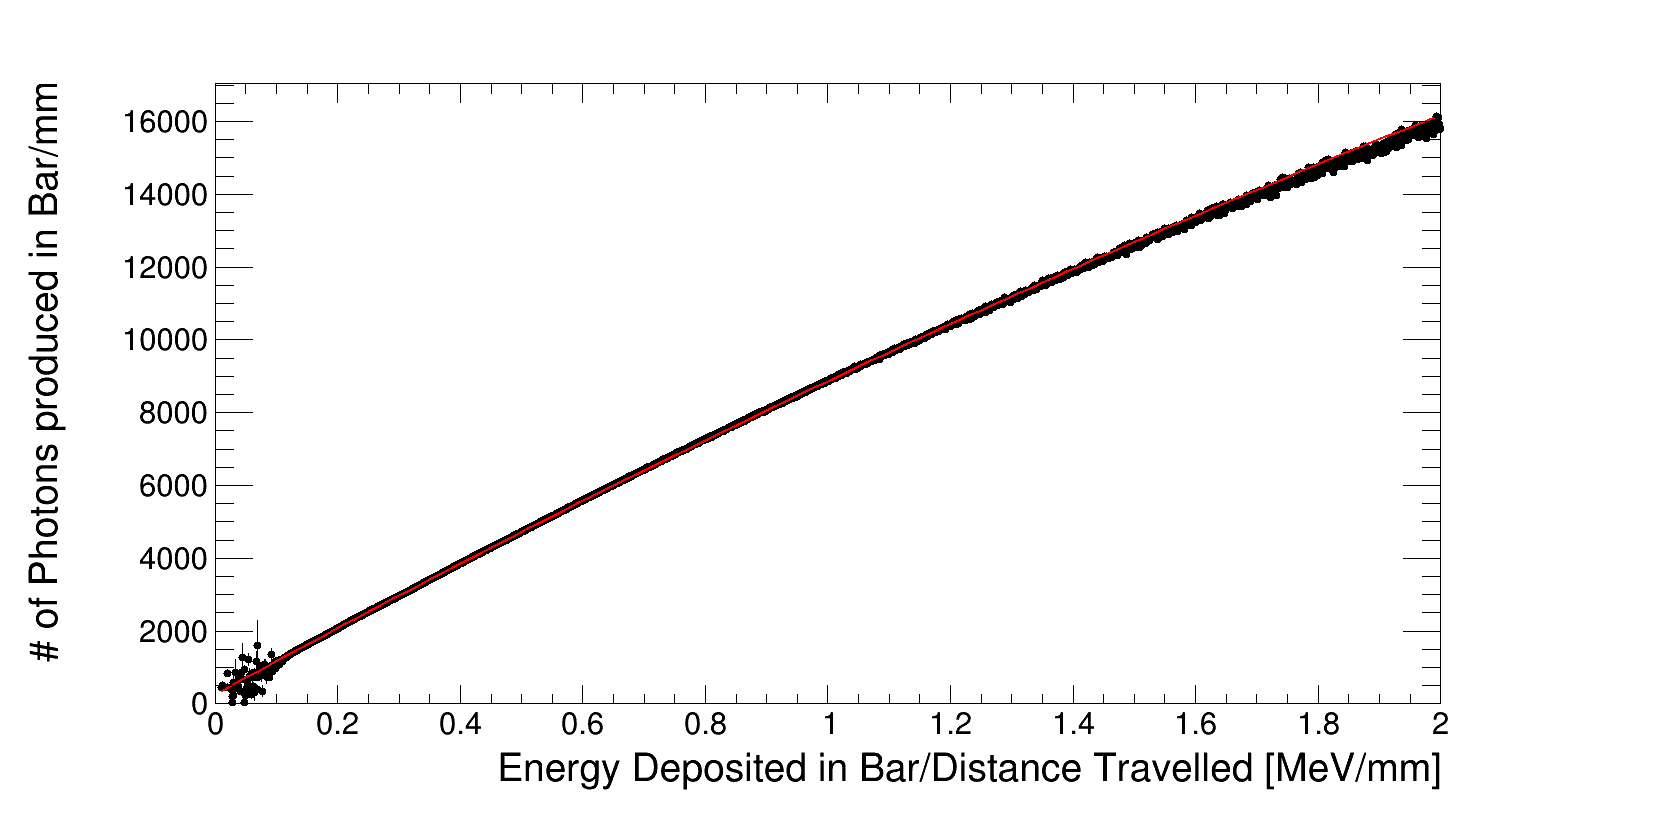
\includegraphics[width=\linewidth]{Appendix4/Figs/newNewDldxVsDeDx/e+_dedxVsdldxFitFine.png}
 \captionof{figure}[dL/dx vs dE/dx 2$^\textrm{nd}$ order polynomial ``slice'' model approximation for positrons.]{dL/dx vs dE/dx fit using the approximation $\Delta L$/$\Delta x$ vs $\Delta E$/$\Delta x$ from the ``slice model'' simulation of scintillator for 2E7 simulated $e^+$ particles, $\chi^2$/NDF = 31.0016. A $^\textrm{nd}$ order polynomial fit is used between 0\,MeV -- 2\,MeV to accurately quantify the effect at low values of dE/dx.} 
 \label{fig:slice_Positron_fine_dl_dx}
\end{figure}
